\documentclass{standalone}
\usepackage{tikz}

\begin{document}

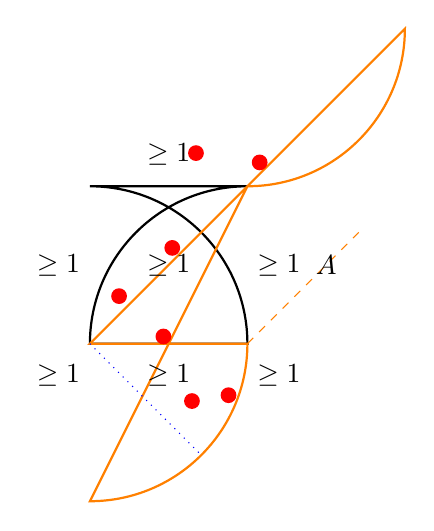
\begin{tikzpicture}[scale=2]
    % Define coordinates for the points
    \coordinate (A) at (0,0);
    \coordinate (B) at (1,0);
    \coordinate (C) at (1,1);
    \coordinate (D) at (0,1);
    
    % Draw the outer boundary of the region A
    \draw[thick] (A) -- (B) arc (0:90:1) -- (C) arc (90:180:1) -- cycle;
    
    % Draw the inner boundary of the region A
    \draw[thick, orange] (A) -- (B) arc (0:-90:1) -- (C) arc (-90:0:1) -- cycle;
    
    % Draw the dashed line
    \draw[dashed, orange] (B) -- ++(45:1);
    
    % Draw the dotted line
    \draw[dotted, blue] (A) -- ++(-45:1);
    
    % Mark the points with red stars
    \foreach \i in {1,...,7} {
        \fill[red] ({rand*1+0.5},{rand*1+0.5}) circle (0.05);
    }
    
    % Label the regions
    \node at (0.5, 1.2) {$\geq 1$};
    \node at (0.5, -0.2) {$\geq 1$};
    \node at (-0.2, 0.5) {$\geq 1$};
    \node at (1.2, 0.5) {$\geq 1$};
    \node at (1.2, -0.2) {$\geq 1$};
    \node at (-0.2, -0.2) {$\geq 1$};
    \node at (0.5, 0.5) {$\geq 1$};
    
    % Label the set A
    \node at (1.5, 0.5) {$A$};
\end{tikzpicture}

\end{document}